Our intention here is to elaborate on the ECG and EHR data available within the MEMIC-IV database, with special attention on the signal and text preprocessing techniques. To begin with, raw ECG signals are subjected to signal preprocessing which incorporates basic steps of noise filtering, physiological signals artificially removing the non-physiological interferences, data shaping into segments of manageable sizes, data scaling, and aligning the signals through re-referencing. On the other hand, the EHR which is usually in the prose format also undergoes text cleaning before being analyzed using text processing techniques involving conversion of uppercase letters to lowercase, segmenting or breaking down the text into the smallest possible words, eliminating auxiliary words and lemmatization or stemming which entails the reduction of a specific word to its base or root. To cope with the lack of data, i.e. introduce imputation, use resolving discrepancies between variable types, and adjust the length of data entries so that all data is the same length, by either cutting excess data or adding additional irrelevant data to the shorter entries. After data processing, ECG and EHR data are fused, and features a built on top of this data to extract informative attributes, for example, for training supervised machine learning, deep learning models, or reinforcement learning. The following steps include selecting a model, training this model, and adjusting hyperparameters for the chosen algorithm. The last stage consists of preparing the resulting model for deployment which enables its use for machine learning model usage to help identify outlying heart signals given the processed EHR and ECG data.
\vspace{0.5cm}


Here is the simple work flow chart given. 

\begin{figure}[ht]
\centering
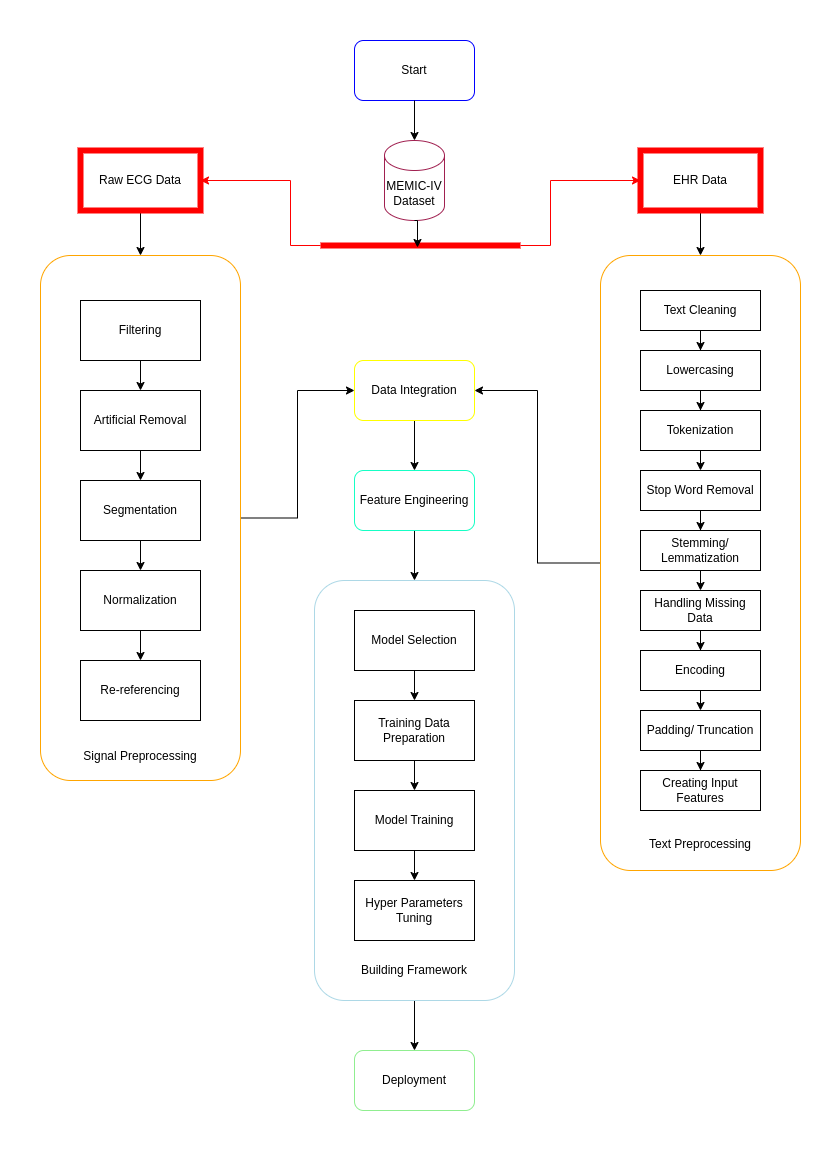
\includegraphics[scale=0.5]{images/workplan.png}
\caption{Workflow}
\label{fig:x Workflow}
\end{figure}